\documentclass{article}
\usepackage{mainPoly}

\title{Suites géométriques}
\date{}
\author{Terminale STMG2}

\begin{document}
\maketitle

\section{Définition}
\begin{tcolorbox}
\begin{definition}
Soit $a \in \R_+$ et $q \in \R_+^*$. On appelle \textbf{suite géométrique à termes positifs} de premier terme $a$ et de raison $q$ une suite $(u_n)_{n \in \N}$ définie par la relation de récurrence suivante :
\begin{equation*}
\begin{cases}
u_0 &= a\\
u_{n+1} &= u_n \times q
\end{cases}
\end{equation*}
\end{definition}
\end{tcolorbox}
\begin{remark}
\hfill
\begin{itemize}
\item De la même manière qu'une suite arithmétique consiste à ajouter la même quantité à chaque étape, une suite géométrique consiste à multiplier par une même quantité à chaque étape.
\item Ici, on impose que la raison soit strictement positive ($\in \R_+^*$).
\end{itemize}
\end{remark}
\begin{example}
Compléter les schémas suivants décrivant des suites géométriques :
\begin{enumquestions}
\item $a = 5$ et $q = 2$
\begin{center}
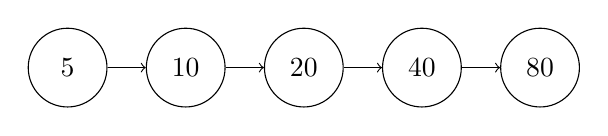
\begin{tikzpicture}
\node[draw, circle, minimum size=1cm] (0) at (0,0) {$5$};
\node[draw, circle, minimum size=1cm] (1) at (1.5,0) {$10$};
\node[draw, circle, minimum size=1cm] (2) at (3,0) {$20$};
\node[draw, circle, minimum size=1cm] (3) at (4.5,0) {$40$};
\node[draw, circle, minimum size=1cm] (4) at (6,0) {$80$};
\draw[->] (0) -- (1); 
\draw[->] (1) -- (2); 
\draw[->] (2) -- (3);
\draw[->] (3) -- (4);
\end{tikzpicture}
\end{center}
\item $a = 64$ et $q = 0.5$
\begin{center}
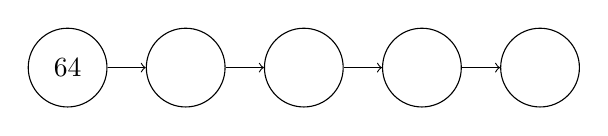
\begin{tikzpicture}
\node[draw, circle, minimum size=1cm] (0) at (0,0) {$64$};
\node[draw, circle, minimum size=1cm] (1) at (1.5,0) {$ $};
\node[draw, circle, minimum size=1cm] (2) at (3,0) {$ $};
\node[draw, circle, minimum size=1cm] (3) at (4.5,0) {$ $};
\node[draw, circle, minimum size=1cm] (4) at (6,0) {$ $};
\draw[->] (0) -- (1); 
\draw[->] (1) -- (2); 
\draw[->] (2) -- (3);
\draw[->] (3) -- (4);
\end{tikzpicture}
\end{center}
\item $a = 1234$ et $q = 0.1$
\begin{center}
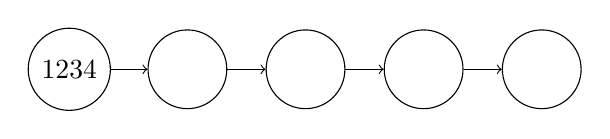
\begin{tikzpicture}
\node[draw, circle, minimum size=1cm] (0) at (0,0) {$1234$};
\node[draw, circle, minimum size=1cm] (1) at (1.5,0) {$ $};
\node[draw, circle, minimum size=1cm] (2) at (3,0) {$ $};
\node[draw, circle, minimum size=1cm] (3) at (4.5,0) {$ $};
\node[draw, circle, minimum size=1cm] (4) at (6,0) {$ $};
\draw[->] (0) -- (1); 
\draw[->] (1) -- (2); 
\draw[->] (2) -- (3);
\draw[->] (3) -- (4);
\end{tikzpicture}
\end{center}
\end{enumquestions}
\end{example}
\begin{tcolorbox}
\begin{definition}[Formule explicite]
Soit $(u_n)_{n \in \N}$ une suite géométrique de premier terme $u_0 = a$ et de raison $q \in \R_+^*$. Alors, pour tout $n \in \N$, on a
\begin{equation*}
u_n = a \times q^n
\end{equation*}
\end{definition}
\end{tcolorbox}
\begin{example}
Pour chacun des exemples précédents, donner directement $u_{10}$.
\vspace*{0.2cm}

\emptybox{4cm}
\end{example}
\newpage

\section{Étude d'une suite géométrique}
\begin{tcolorbox}
\begin{proposition}
Soit $(u_n)_{n \in \N}$ une suite géométrique à termes positifs de raison $q > 0$.
\begin{itemize}
\item Si $q < 1$, alors $(u_n)_{n \in \N}$ est décroissante. 
\item Si $q > 1$, alors $(u_n)_{n \in \N}$ est croissante. 
\item Si $q = 1$, alors $(u_n)_{n \in \N}$ est constante. 
\end{itemize}
\end{proposition}
\end{tcolorbox}
\begin{example}
Soit $(u_n)_{n \in \N}$ une suite géométrique de premier terme $u_0 = 4$ et de raison $q$. Donner une valeur $q_1$ à $q$ pour que $(u_n)_{n \in \N}$ soit croissante, puis une valeur $q_2$ à $q$ pour que $(u_n)_{n \in \N}$ soit décroissante. Tester vos choix en observant les premiers termes de la suite.
\vspace*{0.5cm}

\emptybox{4cm}
\end{example}
\section{Moyenne géométrique}
\begin{tcolorbox}
\begin{definition}
Soit $x$ et $y$ deux nombres positifs. Alors la \textbf{moyenne géométrique} de $x$ et $y$ est donnée par
\begin{equation*}
\sqrt{xy}
\end{equation*}        
\end{definition}
\end{tcolorbox}
\begin{proposition}
Soit $(u_n)_{n \in \N}$ une suite géométrique à termes positifs. Alors, pour tout $n > 1$, on a
\begin{equation*}
u_n = \sqrt{u_{n-1}u_{n+1}}
\end{equation*}
\end{proposition}
\begin{example}
Soit $(u_n)_{n \in \N}$ une suite géométrique à termes positifs, telle que $u_9 = 5$ et $u_{11} = 320$. Calculer $u_{10}$, puis en déduire la raison de cette suite.
\vspace*{0.5cm}

\emptybox{3cm}
\end{example}
\end{document}